\chapter{Scheduling}

\section{The scheduling problem}

The scheduler decides which ready thread runs next on each CPU. We start with a simplified
model of \textbf{jobs}: each job $j$ has an \textbf{arrival time} $a_j$ and a \textbf{run time}
$r_j$, and is CPU-bound (no blocking). Metrics for a schedule:

\begin{description}
  \item[Turnaround time] $t_j - a_j$, where $t_j$ is the completion time.
  \item[Response time] $s_j - a_j$, where $s_j$ is when the job first runs.
  \item[Throughput] jobs completed per unit time.
  \item[Fairness] each job gets a reasonable share; no \textbf{starvation} (a job never runs).
\end{description}
Usually we minimize \emph{average} turnaround or response time. Interactive systems care about
response time; batch systems about turnaround and throughput.

Running example used below:
\begin{center}
\begin{tabular}{@{}ccc@{}}
\toprule
Job & Arrival & Run time \\
\midrule
$J_1$ & 0 & 5 \\
$J_2$ & 0 & 8 \\
$J_3$ & 0 & 3 \\
$J_4$ & 5 & 2 \\
\bottomrule
\end{tabular}
\end{center}

\section{First come, first served (FCFS/FIFO)}

Run jobs in arrival order to completion (ties in index order). Non-preemptive.

\begin{center}
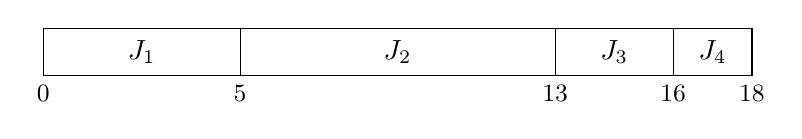
\begin{tikzpicture}[x=0.5cm,y=0.6cm]
  \foreach \s/\e/\n in {0/5/$J_1$,5/13/$J_2$,13/16/$J_3$,16/18/$J_4$}
    \draw (\s,0) rectangle node{\n} (\e,1);
  \foreach \t in {0,5,13,16,18} \node[below,font=\small] at (\t,0) {\t};
\end{tikzpicture}
\end{center}
Turnaround: $5, 13, 16, 13$ $\Rightarrow$ average $47/4 = 11.75$. Short jobs stuck behind long ones
(\textbf{convoy effect}).

\section{Round robin (RR)}

Preemptive FCFS: each job runs for at most a quantum $q$, then goes to the back of the ready
queue. With $q=2$ (a job arriving at time $t$ is enqueued before a job preempted at $t$):

\begin{center}
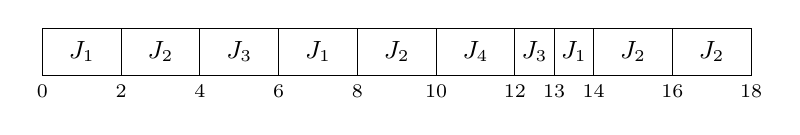
\begin{tikzpicture}[x=0.5cm,y=0.6cm]
  \foreach \s/\e/\n in {0/2/1,2/4/2,4/6/3,6/8/1,8/10/2,10/12/4,12/13/3,13/14/1,14/16/2,16/18/2}
    \draw (\s,0) rectangle node[font=\small]{$J_{\n}$} (\e,1);
  \foreach \t in {0,2,4,6,8,10,12,13,14,16,18} \node[below,font=\scriptsize] at (\t,0) {\t};
\end{tikzpicture}
\end{center}
Turnaround: $J_1 = 14$, $J_2 = 18$, $J_3 = 13$, $J_4 = 12-5 = 7$ $\Rightarrow$ average $13$.
Response times are much better ($0, 2, 4, 5$ vs.\ FCFS $0,5,13,11$). RR trades turnaround for
response time. Quantum choice: too small $\Rightarrow$ context-switch overhead; too large
$\Rightarrow$ degenerates into FCFS.

\section{Shortest job first (SJF)}

Non-preemptive: when the CPU becomes free, run the ready job with the smallest run time.

\begin{center}
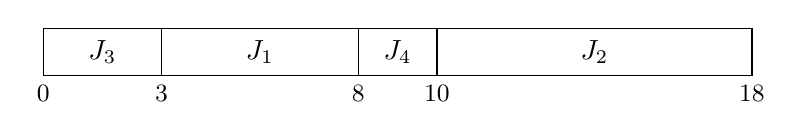
\begin{tikzpicture}[x=0.5cm,y=0.6cm]
  \foreach \s/\e/\n in {0/3/$J_3$,3/8/$J_1$,8/10/$J_4$,10/18/$J_2$}
    \draw (\s,0) rectangle node{\n} (\e,1);
  \foreach \t in {0,3,8,10,18} \node[below,font=\small] at (\t,0) {\t};
\end{tikzpicture}
\end{center}
Turnaround: $J_3=3$, $J_1=8$, $J_4=5$, $J_2=18$ $\Rightarrow$ average $34/4 = 8.5$.

\begin{theorem}
If all jobs arrive at the same time, SJF minimizes average turnaround time.
\end{theorem}
\begin{proof}[Sketch]
Running jobs in order $r_{(1)} \le \dots \le r_{(n)}$, the total turnaround is
$\sum_k (n-k+1) r_{(k)}$: the $k$-th job delays itself and all later jobs. An exchange argument
shows any adjacent pair out of order can be swapped to reduce the sum.
\end{proof}

\section{Shortest remaining time first (SRTF)}

Preemptive SJF: when a job arrives, if its run time is less than the remaining time of the
running job, preempt. In the example, at $t=5$, $J_1$ (started at 3) has 3 remaining and $J_4$
needs 2, so $J_4$ preempts:
\begin{center}
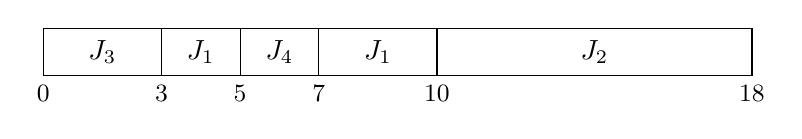
\begin{tikzpicture}[x=0.5cm,y=0.6cm]
  \foreach \s/\e/\n in {0/3/$J_3$,3/5/$J_1$,5/7/$J_4$,7/10/$J_1$,10/18/$J_2$}
    \draw (\s,0) rectangle node{\n} (\e,1);
  \foreach \t in {0,3,5,7,10,18} \node[below,font=\small] at (\t,0) {\t};
\end{tikzpicture}
\end{center}
Turnaround: $3, 10, 2, 18$ $\Rightarrow$ average $33/4 = 8.25$.

\begin{important}[SJF/SRTF in practice]
They are optimal for turnaround but (1) need to know run times in advance and (2) can
\textbf{starve} long jobs if short jobs keep arriving. Real schedulers estimate the next CPU
burst from history, e.g.\ exponential averaging $\tau_{n+1} = \alpha t_n + (1-\alpha)\tau_n$.
\end{important}

\section{Real threads: CPU bursts and I/O}

Real threads alternate CPU \emph{bursts} with blocking for I/O. \textbf{Interactive} (I/O-bound)
threads have short bursts and need good response time; \textbf{CPU-bound} threads have long bursts.
Good schedulers favour I/O-bound threads: they quickly issue I/O and block, keeping devices
busy while CPU-bound work fills the gaps. Many systems also use \textbf{priorities}; strict
priority scheduling can starve low-priority threads, so priorities are often adjusted
dynamically (\emph{aging}).

\section{Multi-level feedback queue (MLFQ)}

MLFQ approximates SJF without knowing run times, by learning from behaviour.

\begin{itemize}
  \item There are $n$ round-robin queues $Q_n$ (highest priority) $\dots Q_1$ (lowest);
    lower-priority queues often have longer quanta.
  \item Always run a thread from the highest non-empty queue.
  \item A new thread enters the top queue.
  \item If a thread uses its whole quantum (CPU-bound), it is \textbf{demoted} one level.
  \item If a thread blocks before its quantum expires (interactive), it stays (or is promoted).
  \item To prevent starvation and adapt to phase changes, periodically \textbf{boost} all
    threads back to the top queue.
\end{itemize}
Gaming: a thread that yields just before its quantum ends could stay on top forever; a fix is to
charge accumulated CPU time at each level, not just per quantum. MLFQ-style schedulers were used
in BSD Unix, Windows NT and Solaris.

\section{Linux Completely Fair Scheduler (CFS)}

CFS aims to give each thread a share of the CPU proportional to its \textbf{weight}, which is
derived from its \emph{nice} value (lower nice, higher weight; each nice step is about a
$1.25\times$ change).

\begin{itemize}
  \item Each thread tracks its \textbf{virtual runtime}:
    \[ \text{vruntime} \mathrel{+}= \text{actual runtime} \times \frac{w_0}{w_i}, \]
    where $w_0$ is the weight of nice level 0. Higher-weight threads accumulate vruntime more
    slowly.
  \item The scheduler always runs the thread with the \emph{smallest} vruntime; ready threads
    are kept in a red-black tree ordered by vruntime ($\bigO(\log n)$ insert, $\bigO(1)$
    leftmost lookup with caching).
  \item The time slice is computed from a target latency (e.g.\ 20\,ms, the period in which
    every ready thread should run once) divided in proportion to weights, with a minimum
    granularity so slices do not become tiny.
  \item A thread that wakes after sleeping gets its vruntime set close to the current minimum,
    so it runs soon (good response) but cannot claim credit for the whole time it slept.
\end{itemize}

\begin{example}
Two threads with weights 2 and 1 (sum 3), target latency 30\,ms: they get slices of 20\,ms and
10\,ms. After both run once, actual runtime $20$ and $10$, vruntime increments
$20 \cdot w_0/2$ and $10 \cdot w_0/1$ --- equal when $w_0 = 1$: both are ``fair''.
\end{example}

\section{Multicore scheduling}

\begin{description}
  \item[Single shared ready queue] Any core takes the next thread from one global queue. Simple
    and naturally load balanced, but the queue lock is a scalability bottleneck, and threads
    hop between cores, losing \textbf{cache affinity}.
  \item[Per-core ready queues] Each core schedules from its own queue. Scales well, and a thread
    keeps running on the same core, so its data stays warm in that core's caches (and TLB).
    Problem: \textbf{load imbalance} (one core idle while another has many threads). Fix:
    \emph{load balancing} by migrating threads --- push migration (a periodic balancer moves
    threads) or \textbf{work stealing}/pull migration (an idle core steals from a busy one).
    Migration costs cache warmth, so it is done sparingly.
\end{description}

\begin{aside}
Cache affinity: after a thread runs on core $c$, its working set is in $c$'s L1/L2 cache.
Moving it to another core means refetching that data from memory (or a shared L3), which can
cost much more than a context switch itself. Linux CFS uses per-core run queues with periodic
balancing across a hierarchy of \emph{scheduling domains} (hyperthreads, cores, sockets/NUMA
nodes).
\end{aside}

\section*{Summary}
\begin{center}
\begin{tabular}{@{}lll@{}}
\toprule
Policy & Preemptive? & Notes \\
\midrule
FCFS & no & simple, convoy effect \\
RR & yes & good response; quantum trade-off \\
SJF & no & optimal avg turnaround (same arrivals); needs run times; starvation \\
SRTF & yes & optimal avg turnaround; starvation \\
MLFQ & yes & learns burst behaviour; priority boost avoids starvation \\
CFS & yes & weighted fair share via vruntime and a red-black tree \\
\bottomrule
\end{tabular}
\end{center}
Multicore: per-core queues for scalability and cache affinity, plus load balancing.
